\section{Προεπεξεργασία Δεδομένων}
\noindent
Το επόμενο στάδιο του συστήματος εκτίμησης DOA, είναι η προεπεξεργασία των συμπιεσμένων αμφιωτικών παραμέτρων, ώστε να μπορούν να χρησιμοποιηθούν για την εκπαίδευση ενός ΝΝ. Στη μηχανική μάθηση, η διαδικασία της προεπεξεργασίας, εκτιμάται ότι είναι τόσο σημαντική όσο και η διαδικασία της κατασκευής του μοντέλου. Παρόλα αυτά όμως, λόγω της πρόσφατης άνθησης του τομέα της μηχανικής μάθησης, δεν υπάρχει αρκετή εμπειρία πάνω σε αυτόν και κατ' επέκταση δεν είναι γνωστός ο καλύτερος τρόπος προεπεξεργασίας των δεδομένων, ανάλογα με τον τύπο τους. Αν και υπάρχουν μερικές τεχνικές οι οποίες είναι ευρέως αποδεκτό ότι παρέχουν καλά αποτελέσματα, επί το πλείστον, οι ερευνητές προσεγγίζουν το πρόβλημα μέσω trial and error.

Μια από τις ευρέως γνωστές τεχνικές προεπεξεργασίας δεδομένων, είναι αυτή της κανονικοποίησης των τιμών των παραμέτρων, ώστε να αποφευχθεί ο κορεσμός του δικτύου όταν προκύπτουν πολύ μεγάλα βάρη στις συνάψεις. Με αυτόν τον τρόπο επιταχύνεται επίσης η διαδικασία της εκπαίδευσης του μοντέλου \cite{Sola1997,Lecun2012}. Εδώ η κανονικοποίηση, έγινε στο κλειστό διάστημα $[-1,1]$, και κρίθηκε πως είναι απαραίτητη λόγω της μεγάλης διαφοράς τάξεως μεγέθους μεταξύ των τιμών της παραμέτρου ILD, η οποία μετριέται σε dB, και της παραμέτρου ITD, η οποία μετριέται σε msec. Με αυτόν τον τρόπο υποδεικνύεται στο μοντέλο, ότι οι παράμετροι πρέπει να αντιμετωπιστούν με την ίδια βαρύτητα. 

Τα προφίλ των παραμέτρων, με διαστάσεις $[2,L]$, μετασχηματίζονται σε διανύσματα γραμμής, με διαστάσεις $[1,2L]$, όπως φαίνεται στην Εξίσωση \ref{eq:profile_flattening}. Τα δύο διανύσματα γραμμής διαστάσεων $[1,2L]$, τελικά συνδυάζονται στο διάνυσμα που θα αποτελέσει την είσοδο του νευρωνικού, με ένα τυπικό παράδειγμα να φαίνεται στο Σχήμα \ref{fig:final_profile}. Σημειώνεται πως τα δεδομένα μετά την προεπεξεργασία χάνουν τη φυσική σημασία τους. 
\begin{CEquation}
\begin{split}
    Input\;Vector[1:L] = Profile[1,L]\\
    Input\;Vector[L+1:2L] = Profile[2,L]
    \label{eq:profile_flattening}
\end{split}
\end{CEquation}
Από τα 7917 διαφορετικά διανύσματα που υπολογίζονται, το 80\% χρησιμοποιείται για την εκπαίδευση του νευρωνικού, το 10\% χρησιμοποιείται για validation, και το υπόλοιπο 10\% για testing. Κάθε διάνυσμα είναι μοναδικό, και αντιστοιχεί σε μία μετάθεση DOA-σήματος εισόδου-δωματίου. Η διαδικασία του διαχωρισμού σε train-validation-test data γίνεται με τυχαίο τρόπο, ώστε τα αποτελέσματα να είναι αξιόπιστα και γενικεύσιμα.

\begin{figure}[h]
  \centering
  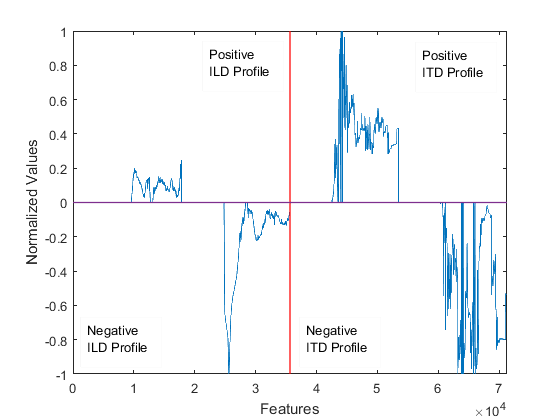
\includegraphics[width=\textwidth]{images/final_profile.png}
  \caption{Τυπικό παράδειγμα κανονικοποιημένου διανύσματος εισόδου στο ΝΝ από τις αμφιωτικές παραμέτρους για συγκεκριμένη γωνία άφιξης.}
  \label{fig:final_profile}
\end{figure}